\section{炉石传说人工智能}
\label{section:HearthstoneAI}
\subsection{炉石传说基本规则}
\label{section:HearthstoneRule}

《炉石传说:魔兽英雄传》,简称“炉石传说”,是由暴雪娱乐推出的一款免费线上卡牌游戏。
炉石传说的世界观依托于暴雪推出的另一款经典游戏《魔兽世界》,将魔兽世界中的英雄、职业及其对应的法术技能变成了炉石传说中的卡牌。
炉石传说包括多种游戏模式,有构筑模式、单人模式、竞技场模式和乱斗模式,而本论文只考虑其中的构筑模式。
在构筑模式中,玩家可以使用自己预先构筑好的卡组来匹配对手,进行游戏。
玩家在选定卡组对应的英雄职业后,可以在该英雄的所有职业专属卡和中立卡之中精心挑选,构成一副由30张卡牌组成的卡组。

炉石传说的一局对局由两名相互敌对的玩家构成。
一名玩家所拥有的游戏实体包括英雄、英雄能力、英雄武器、法力水晶、手牌、牌堆以及在场的随从。

双方的目标均是将对方英雄的生命值下降至0以下,英雄生命值首先到达0以下的玩家输掉对局,两名英雄的生命值同时到达0以下则双方都输掉对局。
炉石传说的对局采用回合轮换制,两名玩家先后轮流地进入自己的回合。
玩家只能在自己的回合中进行操作,当进入对方的回合时则无法进行任何操作。
在对局开始时会随机决定两名玩家的先后手。
先手玩家可以抽3张牌,并在这3张牌中选择任意的牌将其重新洗入牌堆,再抽牌直到手中有3张牌作为自己的起始手牌。
后手玩家则可以在对局开始时抽4张牌,并在进行同样的选牌过程后将其作为自己的起始手牌。
同时,后手玩家还会额外获得一张“硬币”卡\footnote{硬币:0费用法术卡,使玩家当前回合的法力值+1}。
随后,对局先从先手玩家的回合开始。
在对局中两名玩家都会拥有各自的法力水晶。
双方在对局开始前均不拥有任何法力水晶,但每次回合开始时,玩家均获得一枚额外的法力水晶。
法力水晶的数量代表着玩家在每个回合可支配的法力数,使用手中的卡牌将会消耗法力数,而通常消耗越大的卡牌会有着越强的效果。
在玩家的回合开始时,玩家从牌堆中抽一张牌,且所有法力水晶将重新充满。
进入己方回合后,玩家即可任意进行操作,包括使用卡牌、命令随从和英雄攻击以及使用英雄能力。
不同的卡牌有着不同的效果。按类别来分的话,可以分为法术卡、随从卡和武器卡,分别可用于使用法术、召唤随从或为英雄装备武器以进行攻击。
正如前文所说,消耗越大的卡牌意味着越强的效果,也就是越强的法术、越强的随从和越强的武器。
英雄能力的使用同样需要消耗一定的法力,且通常每回合只能使用一次。
与卡牌不同的是,卡牌在使用过后便会消失,某一张卡牌在一场对局中可用的次数是有限的,而英雄能力在整场对局中的使用次数则是没有限制的。
在命令随从和英雄进行攻击时,可以对对方的随从或是英雄进行攻击。当攻击对方攻击力不为0的随从时,攻击的随从或英雄会受到对方随从的反击,受到与目标随从攻击力等同的伤害。
随从在生命值下降到0以下时会死亡。考虑到一名玩家同时只能控制7个随从,当达到上限时将无法召唤更多的随从,因此适当地牺牲随从也有一定的战略意义。
通常来讲,同一个英雄或随从在一个回合中都只能攻击一次,合理地选择它们各自的攻击目标和顺序也可能带来截然不同的战术收益。

图\ref{fig:2}给出了炉石传说中一个回合的基本流程。

\begin{figure}[!ht]
\centering
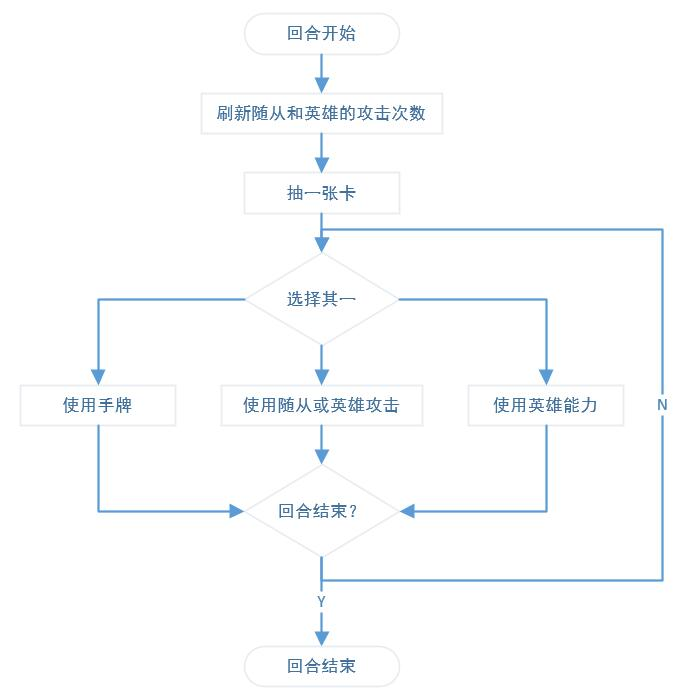
\includegraphics[width=5in,height=5in]{img/Fig2.jpg}
\caption{炉石传说基本流程}
\label{fig:2}
\end{figure}


\subsection{基于规则的智能体}
\label{section:RuleBasedAIPlayers}

在炉石传说中,不同卡组的强度是不一致的,部分卡组会本质上强于其他卡组。
因此,本论文所有的智能体均会使用相同的卡组,卡组的组成如表格\ref{table:TestDeck}所示。
\begin{table}[!ht]
\small
\caption{测试智能体使用的猎人职业卡组}
\label{table:TestDeck}
\begin{tabular}{|l|l|c|c|c|l|c|}
\hline 
名称       & 类型 & 消耗 & 攻击     & 生命     & 效果                                     & 数量 \\
\hline
猎人印记   & 法术 & 0    &          &            & 使一个随从的生命值变为1                  & 2    \\
\hline
奥术射击   & 法术 & 1    &          &            & 造成2点伤害                              & 2    \\
\hline
叫嚣的中士 & 随从 & 1    & 2        & 1          & \textbf{战吼}:本回合中,使一个随从获得+2攻击力 & 2    \\
\hline
狼人渗透者 & 随从 & 1    & 2        & 1          & \textbf{潜行}                                   & 2    \\
\hline
爆炸陷阱   & 法术 & 2    &          &            & \tabincell{ll}{\textbf{奥秘}:&当你的英雄受到攻击时,\\&对所有敌人造成2点伤害} & 2 \\
\hline
冰冻陷阱   & 法术 & 2    &          &            & \tabincell{ll}{\textbf{奥秘}:&当一个敌方随从进攻时,\\&将其移回到所有者手中,\\&并使其法力值消耗增加(2)} & 2 \\
\hline
鬼灵爬行者 & 随从 & 2    & 1        & 2          & \textbf{亡语}:召唤两个1/1的鬼灵蜘蛛 & 2 \\
\hline
鹰角弓     & 武器 & 3    & 3        & 2          & \tabincell{l}{每当有一张你的\textbf{奥秘}牌被揭示时,\\便获得+1耐久度} & 2 \\
\hline
杀戮命令   & 法术 & 3    &          &            & \tabincell{l}{造成3点伤害。\\如果你控制野兽,则改为造成5点伤害} & 2 \\
\hline
关门放狗   & 法术 & 3    &          &            & \tabincell{l}{战场上每有一个敌方随从,\\便召唤一个1/1并具有\textbf{冲锋}的猎犬} & 2 \\
\hline
蜘蛛坦克   & 随从 & 3    & 3        & 4          &                                 & 2 \\
\hline
冰风雪人   & 随从 & 4    & 4        & 5          &                                 & 2 \\
\hline
火车王里艾诺 & 随从 & 5 & 6 & 2 & \textbf{冲锋},\textbf{战吼}:为你的对手召唤两只1/1的雏龙 & 1 \\
\hline
石拳食人魔 & 随从 & 6 & 6 & 7 & & 2 \\
\hline
加兹瑞拉   & 随从 & 7 & 6 & 9 & 每当该随从受到伤害,便获得攻击力翻倍 & 1 \\
\hline
强袭坦克   & 随从 & 8 & 7 & 7 & \textbf{圣盾} & 2 \\
\hline
\end{tabular}
\end{table}

该卡组借鉴了以往出现过的许多胜率稳定的猎人卡组,其中包含的卡牌的法力消耗跨度较大,包括了从消耗小同时体量小的随从卡到消耗大且体量大的随从卡,以及一定的法术卡。其中甚至还包括了一张名为“火车王里艾诺”的传说卡牌。传说卡牌是炉石传说中稀有度最高的卡牌,比起其他卡牌会有着强得多的效果。“火车王里艾诺”对于猎人卡组是一张很经典的卡牌,同时也拥有比其他卡牌更复杂的效果,因此十分适合用于测试智能体对效果较复杂的卡牌的处理能力。

在给定的测试环境下,智能体需要进行的决策包括如下:
\begin{enumerate}
\item 决定使用哪张手牌;
\item 决定使用哪个随从或英雄进行攻击,以及攻击的目标;
\item 决定是否使用英雄能力,以及英雄能力的目标。
\end{enumerate}
除此之外,智能体还需要决定上述操作的先后次序。

英雄或随从的攻击决策是完全信息的:所有可进行攻击的角色和可被攻击的目标都是可见的,攻击后的效果也是确定的。大部分英雄能力使用后的效果也是确定的,但少部分职业的英雄能力本身也存在一定的随机性。手牌使用的决策则是不完全信息的:是否使用某一张手牌还需要考虑下一张可能抽到的牌,因为特定卡牌之间的配合可以在炉石传说之中打出更好的效果;除此之外,对方的手牌和牌堆的信息也是隐藏的,我方手牌的使用同样需要考虑这些信息。

除了一个完全随机的智能体,本文还使用了一个基于规则的智能体进行试验。该智能体会按照预先设定的启发规则进行上述的决策。
首先它会根据对方在场随从和英雄的攻击力计算出对方的场攻。如果对方的场攻数高于当前我方英雄剩余生命值,即我方形势已十分险峻,
那么便会首先决定是否要打出某些满足条件的手牌进行自保,如召唤一个嘲讽\footnote{当对方拥有一个被标记为“嘲讽”的随从时,
我方英雄和随从无法对对方其他随从或英雄进行直接攻击,直到对方所有的嘲讽随从阵亡。}随从。
而后,智能体会根据手牌的优先级打出优先级最高的手牌。对于绝大多数卡牌而言,法力消耗越高的卡牌拥有越高的优先级。
在完成手牌的决策后,智能体会根据规则来判断哪些敌方随从对己方威胁较大。威胁较大的随从包括攻击力或生命值过高的随从。
当存在威胁较大的敌方随从时,智能体将在我方可进行攻击的随从中选取最优的攻击者,以求能以最小的代价杀死该威胁较大的敌方随从\footnote{随从进行攻击时会受到敌方随从的反击。优先以生命值远小于敌方随从攻击力的随从进行攻击可以使得我方生命值较高的的随从得以保留,从而控制损失。}。
当不存在这样的敌方随从时,我方所有可攻击的随从和英雄都会直接攻击敌方英雄,以求通过激进地压低敌方生命值为对方增加压力,从而拉大优势、赢得对局。
最终,如仍有充足的法力剩余,智能体将使用英雄能力。

正如前文所述,炉石传说是很复杂的游戏,如此简单的规则智能体固然无法与人类玩家相提并论。实际上,鉴于炉石传说的受欢迎程度之大,
在进行排名比赛时往往可以在较低的排名中匹配到使用规则智能体进行自动游戏以获益的玩家,即所谓的“脚本”。在与这些脚本进行对战时,
我们的规则智能体往往表现不俗,并在多数情况下取胜。由此,尽管确实无法与人类玩家相提并论,本文使用的规则智能体已具有一定的决策强度。

\subsection{蒙特卡洛智能体}
\label{section:MonteCarloAIPlayers}

除了随机和规则智能体外,本文主要测试的智能体由蒙特卡洛搜索进行实现。具体而言,本文使用的蒙特卡洛智能体实现了可用于解决多臂赌博机问题的UCB1算法\cite{auer2002finite}。
在多臂赌博机问题中,参与者需要在若干个随机出奖的赌博机之间进行选择,而使用UCB1算法能确保参与者在足够多次的尝试后获得最高的收益。

UCB1算法的基本过程如下所述:
\begin{itemize}
\item[初始化] 对每个赌博机各尝试一次;
\item[循环] 选取使得公式
\begin{equation}
\label{eq:UCB}
\bar{x}_j + C\sqrt{\frac{\ln n}{n_j}}
\end{equation}
最大化的赌博机$j$进行尝试。其中$\bar{x}_j$为赌博机$j$过往的平均收益,$C$为一个$0$和$1$之间的常数,决定搜索算法尝试其他赌博机的可能性大小;$n_j$为赌博机$j$过去被尝试的次数,$n=\sum_i n_i$为尝试次数的总和。
\end{itemize}

根据UCB1算法的基本过程,将其应用于炉石传说也并非难事。蒙特卡洛智能体的决策过程基本如下:
\begin{enumerate}
\item 根据当前游戏状态枚举出智能体在当前回合可以进行的所有操作序列;
\item 为每个可进行的操作序列均将游戏模拟至游戏结束,并保存模拟的结果;
\item 进入UCB1算法的循环阶段,使用公式\ref{eq:UCB}选取操作序列并将游戏模拟至游戏结束,然后保存模拟的结果;
\item 在满足一定的预设条件后结束循环,并返回平均收益$\bar{x}_j$最高的操作序列。
\end{enumerate}
